% !TEX TS-program = pdflatex
% !TEX encoding = UTF-8 Unicode
\documentclass[a4paper,twoside,11pt]{article}
\usepackage[polish]{babel}
\usepackage[MeX]{polski}
\usepackage[utf8]{inputenc}
\usepackage{indentfirst,graphicx,amsmath}
\usepackage[left=2cm,top=2cm,right=2cm,nohead]{geometry}
\usepackage{hyperref}
\usepackage{tabularx}
\usepackage{color}
\usepackage{float}
\frenchspacing
\pagestyle{plain}

\makeatletter
\renewcommand\@seccntformat[1]{\csname the#1\endcsname.\quad}
\renewcommand\numberline[1]{#1.\hskip0.7em}
\makeatother

\newenvironment{mylisting}
{\begin{list}{}{\setlength{\leftmargin}{1em}}\item\scriptsize\bfseries}
{\end{list}}

\newenvironment{mytinylisting}
{\begin{list}{}{\setlength{\leftmargin}{1em}}\item\tiny\bfseries}
{\end{list}}

\usepackage{graphicx}
\usepackage{color}

\author{\\ ~ \\ Tomasz Gański \\
Tomasz Gieniusz \\
Bartosz Jankowski\\
Grzegorz Marcinkowski\\
Łukasz Odzioba\\
Jacek Weremko}
\title{\LARGE Wykrywacz zachcianek gastronomicznych}

\begin{document}

\makeatletter

\renewcommand{\maketitle}{
	\begin{titlepage}
		\begin{center}
			\small Politechnika Gdańska \\ Wydział Elektroniki, Telekomunikacji i Informatyki
		\end{center}
		\vspace{3cm}
		\noindent \rule{\linewidth}{0.4mm}
		\begin{center}
			\textsc{
				\huge{Architektura systemu } \\
				\vspace{0.3ex}
				\LARGE{Systemy z Bazą Wiedzy}
			}
			\\
			\vspace{1em}
			\Large{\@title}
		\end{center}
		\rule{\linewidth}{0.4mm}
		\vspace{1em}
		\begin{center}
			\large Autorzy: \@author
		\end{center}
		\vspace{7em}
		\ifpdf
			\begin{tabularx}{\textwidth}{ X X }
				\makebox[0.5\textwidth][l]{
					\hspace{1cm}
					
\includegraphics[width=4cm]{logo_pg}
				}
				&
				\makebox[0.5\textwidth][r]{
					
\includegraphics[width=4cm]{logo_eti}
					\hspace{1cm}
				}
			\end{tabularx}
		\fi
		% Duży odstęp, który powoduje, że stopka z datą pojawia się na dole. Dokładniej wypycha ją
		% poza stronę, ale latex na to nie pozwala i umieszcza ją na końcu strony.
		\vspace*{\stretch{6}}
		\begin{center}
			Gdańsk, \@date \ r.
		\end{center}
	\end{titlepage}
}

\makeatother

\maketitle{}


\tableofcontents

\newpage

\section{Cel projektu}
Celem projektu jest stworzenie systemu doradczego, ułatwiającego życie każdego człowieka. Każdy z nas bywa w sytuacjach, gdy jest głodny lecz niezdecydowany co do konkretnej potrawy. \\ 

System na podstawie wielu parametrów, takich jak wiek użytkownika, aktualna pora dnia, roku, pogoda, itp. będzie w stanie ułatwić użytkownikowi podjęcie decyzji sugerując mu typowe potrawy, które mogą pobudzić jego kubki smakowe.

\section{Technologia}
Projekt zostanie wykonany na platformę mobilną Android (zgodność z wersjami Donut i nowszymi). Wykorzystane zostanie natywne API systemu, a także system AdMob w celu wyświetlania reklam po umieszczeniu aplikacji w Android Market. \\

Aplikacja do działania będzie wymagała dostępu do internetu oraz aktualnej lokacji użytkownika. \\

System uczący będzie zaimplementowany w formie sieci neuronowej której współczynniki będa zapisywane do pamięci trwałej, tak aby zachować jej stan pomiędzy uruchomieniami aplikacji.

\section{Struktura systemu}
\subsection{Struktura sprzętowa}
	\begin{figure}[H]
		\begin{center}
			\scalebox{0.6}{
                                	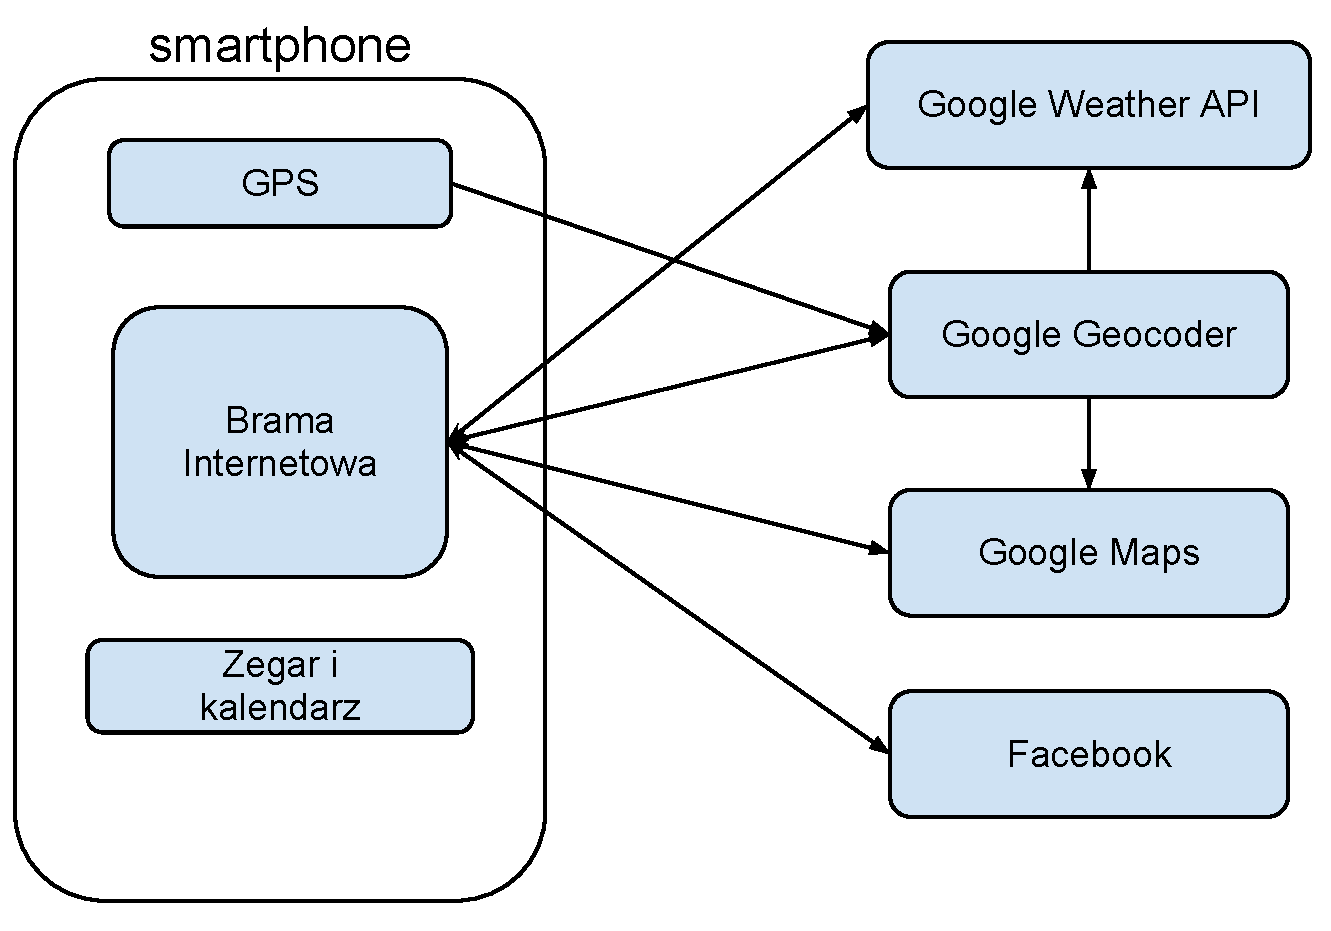
\includegraphics{images/Strukturasprzetowa}
                        	}
           	\end{center}
           	\caption{Diagram komponentów sprzętowych}
	\end{figure}

\subsection{Struktura programowa}
	\begin{figure}[H]
		\begin{center}
			\scalebox{0.5}{
                                	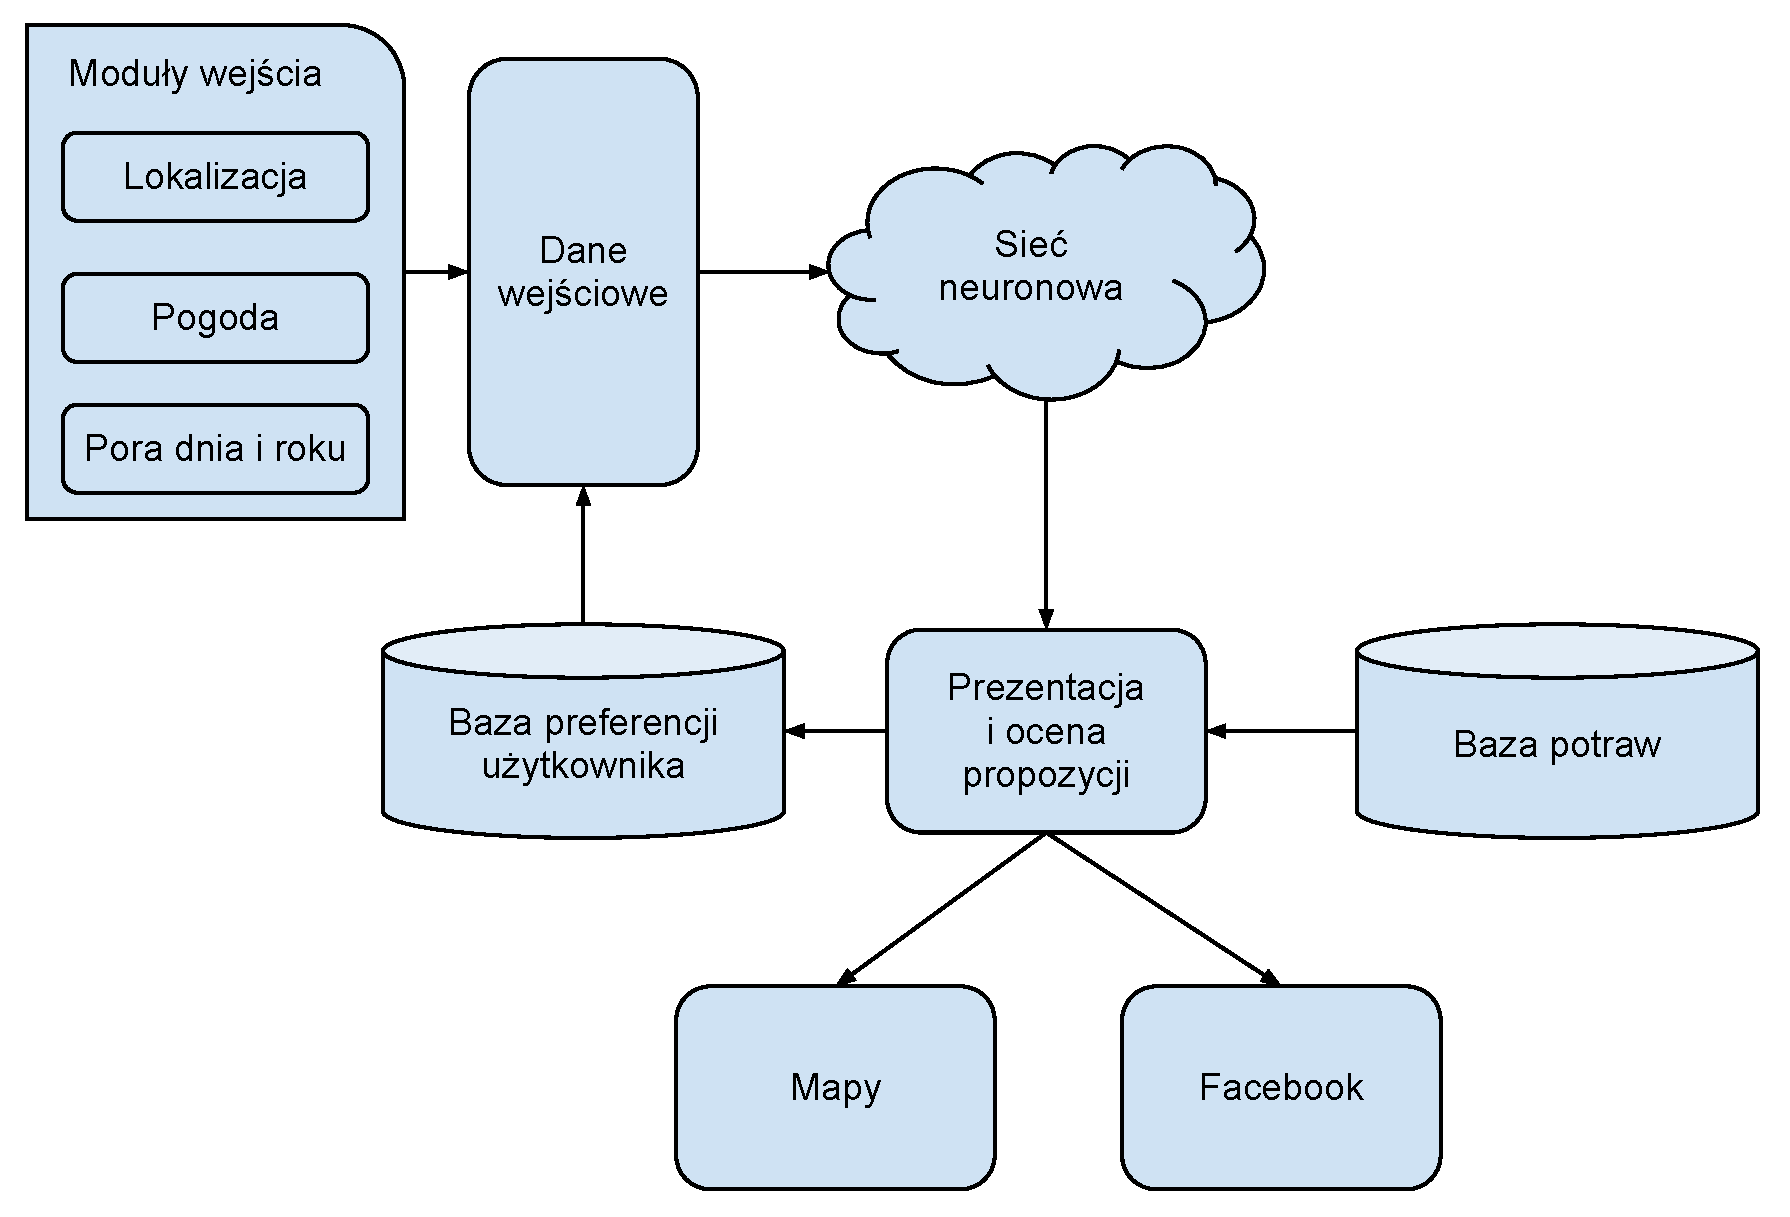
\includegraphics{images/Strukturaprogramowa}
                        	}
           	\end{center}
           	\caption{Diagram komponentów programowych}
	\end{figure}



\section{Komponenty programowe}

\subsection{Moduły wejścia}
Komponent systemu zajmujący się pobraniem danych
\begin{itemize}
	\item lokalizacyjnych
	\item pogodowych
	\item czasowych
\end{itemize}
z API udostepnionego przez system Android.

\subsection{Dane wejściowe}
Celem tego komponentu jest przekonwertowanie oraz wyfiltrowanie danych pobranych przez moduły wejścia do formy akceptowalnej przez sieć neuronową. Dodatkowa warstwa umożliwia wprowadzanie zmian w kodzie komponentów dostarczających dane, bez zmiany interfejsu sieci neuronowej.

\subsection{Baza preferencji użytkownika}
Baza danych zapisana w pamięci trwałej telefonu, przechowująca preferencje użytkownika uzyskane na podstawie jego poprzednich wyborów. Wykorzystywane są one jako współczynniki w sieci neurnowej, dzięki nim sieć może dostosowywać się do  zmieniających się preferencji użytkownika.

\subsection{Baza potraw}
Z góry określona baza dostępnych w systemie potraw wraz z ich oznaczenia pod kątem
\begin{itemize}
	\item rozmiaru (delikatny, mały, średni, duży)
	\item smaku (słony, słodki, kwaśny, nieistotny)
	\item posiłku (śniadanie, obiad, kolacja, nieistotny)
	\item diety (wegetariańska, koszerna, mięsna, nieistotna)
	\item słowa kluczowe oznaczające gdzie można dostać daną potrawę (sklep spożywczy, pizzeria, restauracja meksykańska, itp.)
\end{itemize}

\subsection{Prezentacja i ocena propozycji}
Głównym zadaniem tego komponentu jest zaprezentowanie użytkownikowi propozycji wygenerowanej przy pomocy sieci neuronowej w czytelnej i estetycznej formie. Interfejs będzie intuicyjny a każdy widoczny dla użytkownika ekran powinien zawierać co najwyżej kilka elementów takich jak zdjęcie lub przycisk, tak aby nie został on przytłoczony ilością informacji. 

Zdjęcia produktów będą pobrane z wyszukiwarki obrazów google, dzięki temu użytkownik nie będzie odczuwał monotonii nawet wtedy gdy system zaproponuje mu kilka razy pod rząd tą samą potrawę.
Po prezentacji potrawy użytkownik ma możliwość ocenić trafność przy pomocy dwóch przycisków “Good” i “Bad”. Wybór zostanie przeniesiony do bazy preferencji i będzie miał wpływ na przyszłe działanie sieci neuronowej.

Gdy zaproponowany posiłek będzie tym którego użytkownik naprawdę pragnie, będzie mógł podzielić się swoim wyborem ze znajomymi na Facebooku, a aplikacja zaproponuje mu najbliższe miejsce gdzie może zjeść daną potrawę.

\section{Przegląd przypadków użycia}

\subsection{Pierwsze uruchomienie}
\begin{itemize}
\item Użytkownik włącza aplikacje i przechodzi test potrawa x vs potrawa y
\item Użytkownik włącza aplikacje i pyta co chce zjeść
\item System na podstawie początkowych preferencji oraz innych danych wyznacza dla użytkownika potrawę
\item Użytkownik potwierdza zgodność z jego oczekiwaniami
\item Użytkownik dzieli się swoim wyborem na Facebookui wyszukuje najbliższą restauracje
\end{itemize}

\subsection{Doświadczony użytkownik}
\begin{itemize}
\item Użytkownik włącza aplikacje i pyta co chce zjeść
\item System na podstawie wczesniejszych prefykcjioraz innych danych wyznacza dla użytkownika potrawę
\item Użytkownik nie potwierdza zgodności z jego oczekiwaniami
\item System zapisuje ocenę użytkownika oraz proponuję mu inną potrawę
\item Użytkownik potwierdza zgodność z jego oczekiwaniami
\end{itemize}


\section{Zadania do wykonania}
\begin{itemize}
  \item Dodanie bazy posiłków
  \item Połączenie z Facebookiem
  \item Wstępny research nad predykcją
  \item Interfejs + grafiki
  \item Dopracowanie mapy
  \item Research nad innymi sieciami społecznościowymi
  \item Strona Menu
  \item Opracowanie i wdrożenie metod kontroli umysłów
  \item Dodanie nowych tasków
  \item Siec neuronowa
  \item Opracowanie formatu bazy preferencji
  \item Testy systemu
  \item Przygotowanie raportu z testów
  \item Przygotowanie zbioru uczączego dla SN
  \item Zmienić pobieranie obrazów potraw na losowe z listy zamiast top1
\end{itemize}



\end{document}
